\documentclass[twoside,final]{hcmut-report}
\usepackage{codespace}

% Encodings & symbols
\usepackage{gensymb,textcomp}

% Better tables
\usepackage{array,longtable,multicol,multirow,siunitx,tabularx}

% Better enum
\usepackage{enumitem}

% Graphics
\usepackage{caption,float}
\usepackage[export]{adjustbox}

% References
\usepackage[nameinlink]{cleveref}

% Configurations
\coursename{Deep Learning and Its Applications (CO3133)}
\reporttype{Assignment 3 -- M1 Dataset Proposal}
\title{Multimodal Food Classification on UPMC Food-101}
\advisor{& Lê Thành Sách &}
\stuname{%
  & Trần Gia Lâm (Leader) & 2352670 \\
  & Nguyễn Hữu Cầu & 2352129 \\
}
\reporttime{November 2026}

\setlength{\emergencystretch}{3em}

\begin{document}
\coverpage

\section*{Abstract}
\addcontentsline{toc}{section}{Abstract}
Multimodal food recognition requires integrating visual appearance (dish photographs) with noisy web text (recipe webpage titles) to classify dishes into fine-grained categories. In this Assignment 3 M1 Dataset Proposal for CO3133 (Semester 261, Group G-M10), we propose \textbf{Image--Text Multimodal Classification} on the \textbf{UPMC Food-101} benchmark (101 food categories). Using an automated Exploratory Data Analysis (EDA) pipeline (\texttt{notebooks/A3\_EDA\_Proposal.ipynb}) executed directly on the official \texttt{UPMC-Food-101.zip} archive, we verify all \textbf{86,768} paired records (65,085 official train and 21,683 official test), confirming \textbf{0} missing/corrupt images, \textbf{0} empty texts, and 100\% RGB format.

Our EDA uncovers three key properties that shape our modeling plan: (1) \textbf{14.62\%} of recipe titles contain raw HTML entities requiring \texttt{html.unescape()}; (2) \textbf{72.08\%} of titles contain the exact class phrase while \textbf{27.92\%} do not (including boilerplate artifacts such as \texttt{\#NAME?} appearing 235 times), motivating multimodal fusion; and (3) exact SHA-256 hashing and 64-bit perceptual dHash ($\text{dist} \le 3$) detect 2,491 exact duplicate image groups and 11,698 near-duplicate pairs. Grouping by \texttt{recipe\_id} and duplicate clusters via \texttt{StratifiedGroupKFold} produces a leak-free \textbf{52,068 train / 13,017 validation} split (validation share 19.85\%--20.12\% across all 101 classes, 0 cross-split overlap), while an audit against official \texttt{test} flags 1,018 exact and 4,395 near-duplicate overlaps to be reported separately in M2/M3. Finally, we specify our 4 mandatory models (Image-only \texttt{ConvNeXt-Tiny}, Text-only \texttt{DistilBERT}, Late Concatenation Fusion, and Gated Cross-Modal Attention with Modality Dropout), ablation plan, and a $\sim$12 GPU-hour Google Colab T4 compute budget.

\clearpage
\tableofcontents

\clearpage
\section{Team Responsibilities \& Proposal Status}

\begin{table}[H]
\centering
\caption{Group G-M10 Responsibilities and Contribution Plan (M1--M3)}
\begin{tabularx}{\linewidth}{l X c}
\toprule
\textbf{Member} & \textbf{Planned M1--M3 Responsibilities} & \textbf{Contribution} \\
\midrule
Trần Gia Lâm (2352670) & Dataset proposal design, Image-only \& Improved Multimodal Fusion implementation, ablation \& modality conflict analysis, report integration and submission. & 100\% \\
Nguyễn Hữu Cầu (2352129) & Multimodal EDA pipeline, SHA-256/dHash duplicate auditing \& leakage-free split generation, Text-only \& Simple Fusion baselines, compute logging. & 100\% \\
\bottomrule
\end{tabularx}
\end{table}

\begin{itemize}
    \item \textbf{Approval Status:} Pending Instructor Review (\emph{Approved / Approved with conditions / Rejected}). Main M2/M3 experiments will commence only after approval.
    \item \textbf{Reproducibility Note:} Every quantitative figure and table in this proposal is computed directly from \texttt{UPMC-Food-101.zip} via \texttt{notebooks/A3\_EDA\_Proposal.ipynb} and stored in \texttt{outputs/a3\_eda/summary.json} and \texttt{quality\_checks.json}.
\end{itemize}

\section{Dataset Specification \& Task Definition}

\begin{table}[H]
\centering
\caption{UPMC Food-101 Dataset Specification (Handbook Sections 26--28)}
\begin{tabularx}{\linewidth}{l X}
\toprule
\textbf{Field} & \textbf{Specification} \\
\midrule
Dataset Name & UPMC Food-101 (Wang et al., ICMEW 2015) \\
Source \& Version & Hugging Face Hub \texttt{kkim0451/UPMC-Food101}, v1.0 (\texttt{UPMC-Food-101.zip}, 8,268,462,033 bytes) \\
License & \texttt{apache-2.0} for dataset packaging; underlying web-collected recipe images and titles are used strictly for academic, non-commercial research. \\
Task \& Modalities & Single-label multi-class \textbf{Image--Text Classification} (101 food categories); Modalities: RGB Image + English Recipe Webpage Title. \\
Input \& Output & Input: paired $(\text{Image}, \text{Recipe Title})$ from the same recipe webpage (\texttt{recipe\_id}); Output: 101-class probability distribution $\hat{y} \in \Delta^{100}$. \\
Handbook 28.2 Compliance & \textbf{101 classes} ($\ge 5$ required); \textbf{86,768 valid paired samples} (65,085 official train + 21,683 official test; $\ge 5,000$ required). \\
\bottomrule
\end{tabularx}
\end{table}

\section{Preliminary Pair-Quality \& Multimodal EDA}

Every record in \texttt{train.csv} (65,085) and \texttt{test.csv} (21,683) was verified by decoding its JPEG image inside \texttt{UPMC-Food-101.zip} with PIL, auditing text completeness, HTML entity rates, class-phrase presence, and computing exact SHA-256 and 64-bit perceptual dHash signatures.

\begin{table}[H]
\centering
\caption{Multimodal Pair-Quality and Distribution Audit (Total = 86,768 Records)}
\begin{tabularx}{\linewidth}{l l X}
\toprule
\textbf{Audit Dimension} & \textbf{Observed Value} & \textbf{Preprocessing / Modeling Implication} \\
\midrule
Valid Paired Samples & \textbf{86,768 / 86,768 (100.00\%)} & 0 missing/corrupt images; 0 empty texts; 0 non-RGB images. \\
Image Width (min/med/p90/max) & 120 / \textbf{500} / 1,039 / 2,000 px & Standardize to $224\times 224$ (Resize 256 + Crop). \\
Image Height (min/med/p90/max) & 120 / \textbf{399} / 779 / 2,960 px & Aspect ratios centered near 1.0--1.33. \\
Word Count (min/p10/med/mean/p90/max) & 0 / 4 / \textbf{7} / \textbf{7.50} / 12 / 155 & \texttt{max\_length=64} covers $>99\%$ of titles. \\
HTML Entities in Titles & \textbf{14.62\%} (\texttt{\&\#8217;}, \texttt{\&raquo;}) & Apply \texttt{html.unescape()} before tokenization. \\
Class Phrase in Title & \textbf{72.08\%} yes / \textbf{27.92\%} no & 27.92\% require visual cues or contextual reasoning. \\
Unique Clean Titles & 60,657 (e.g., \texttt{\#NAME?} $\times 235$) & Modality dropout prevents over-reliance on noisy titles. \\
Duplicate Images (SHA-256 / dHash) & \textbf{2,491} groups / \textbf{11,698} pairs & Grouped via Union-Find prior to train/val splitting. \\
\bottomrule
\end{tabularx}
\end{table}

\begin{figure}[H]
    \centering
    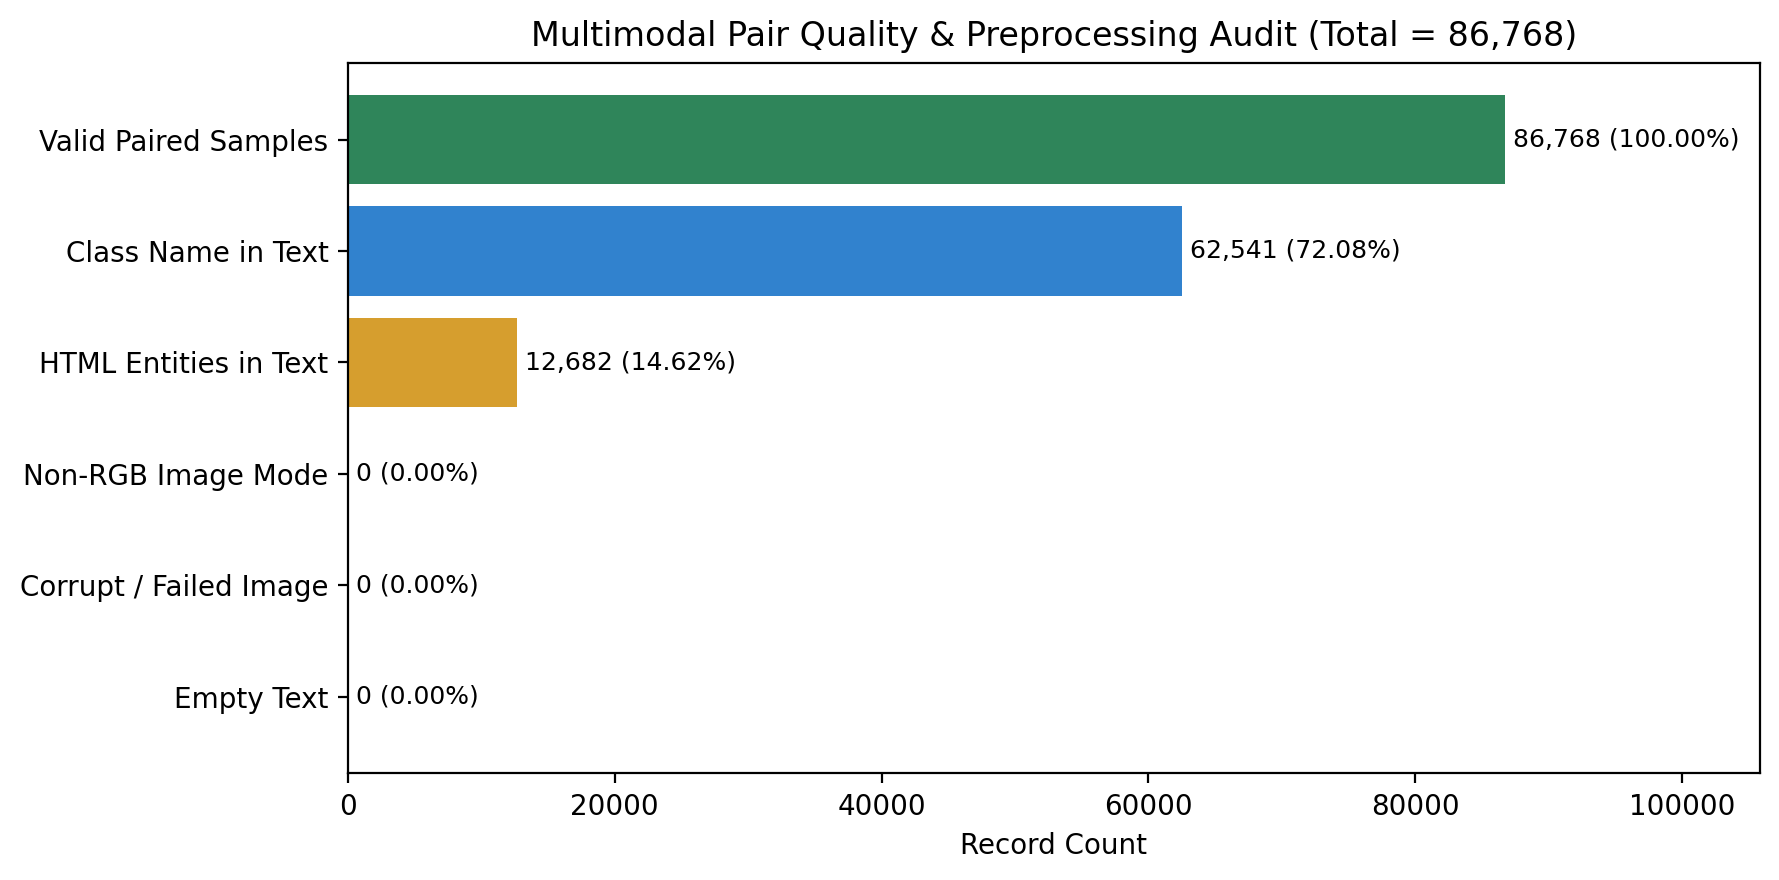
\includegraphics[width=0.90\linewidth]{../outputs/a3_eda/figures/modality_quality_summary.png}
    \caption{Multimodal pair-quality and preprocessing audit across all 86,768 records.}
\end{figure}

\begin{figure}[H]
    \centering
    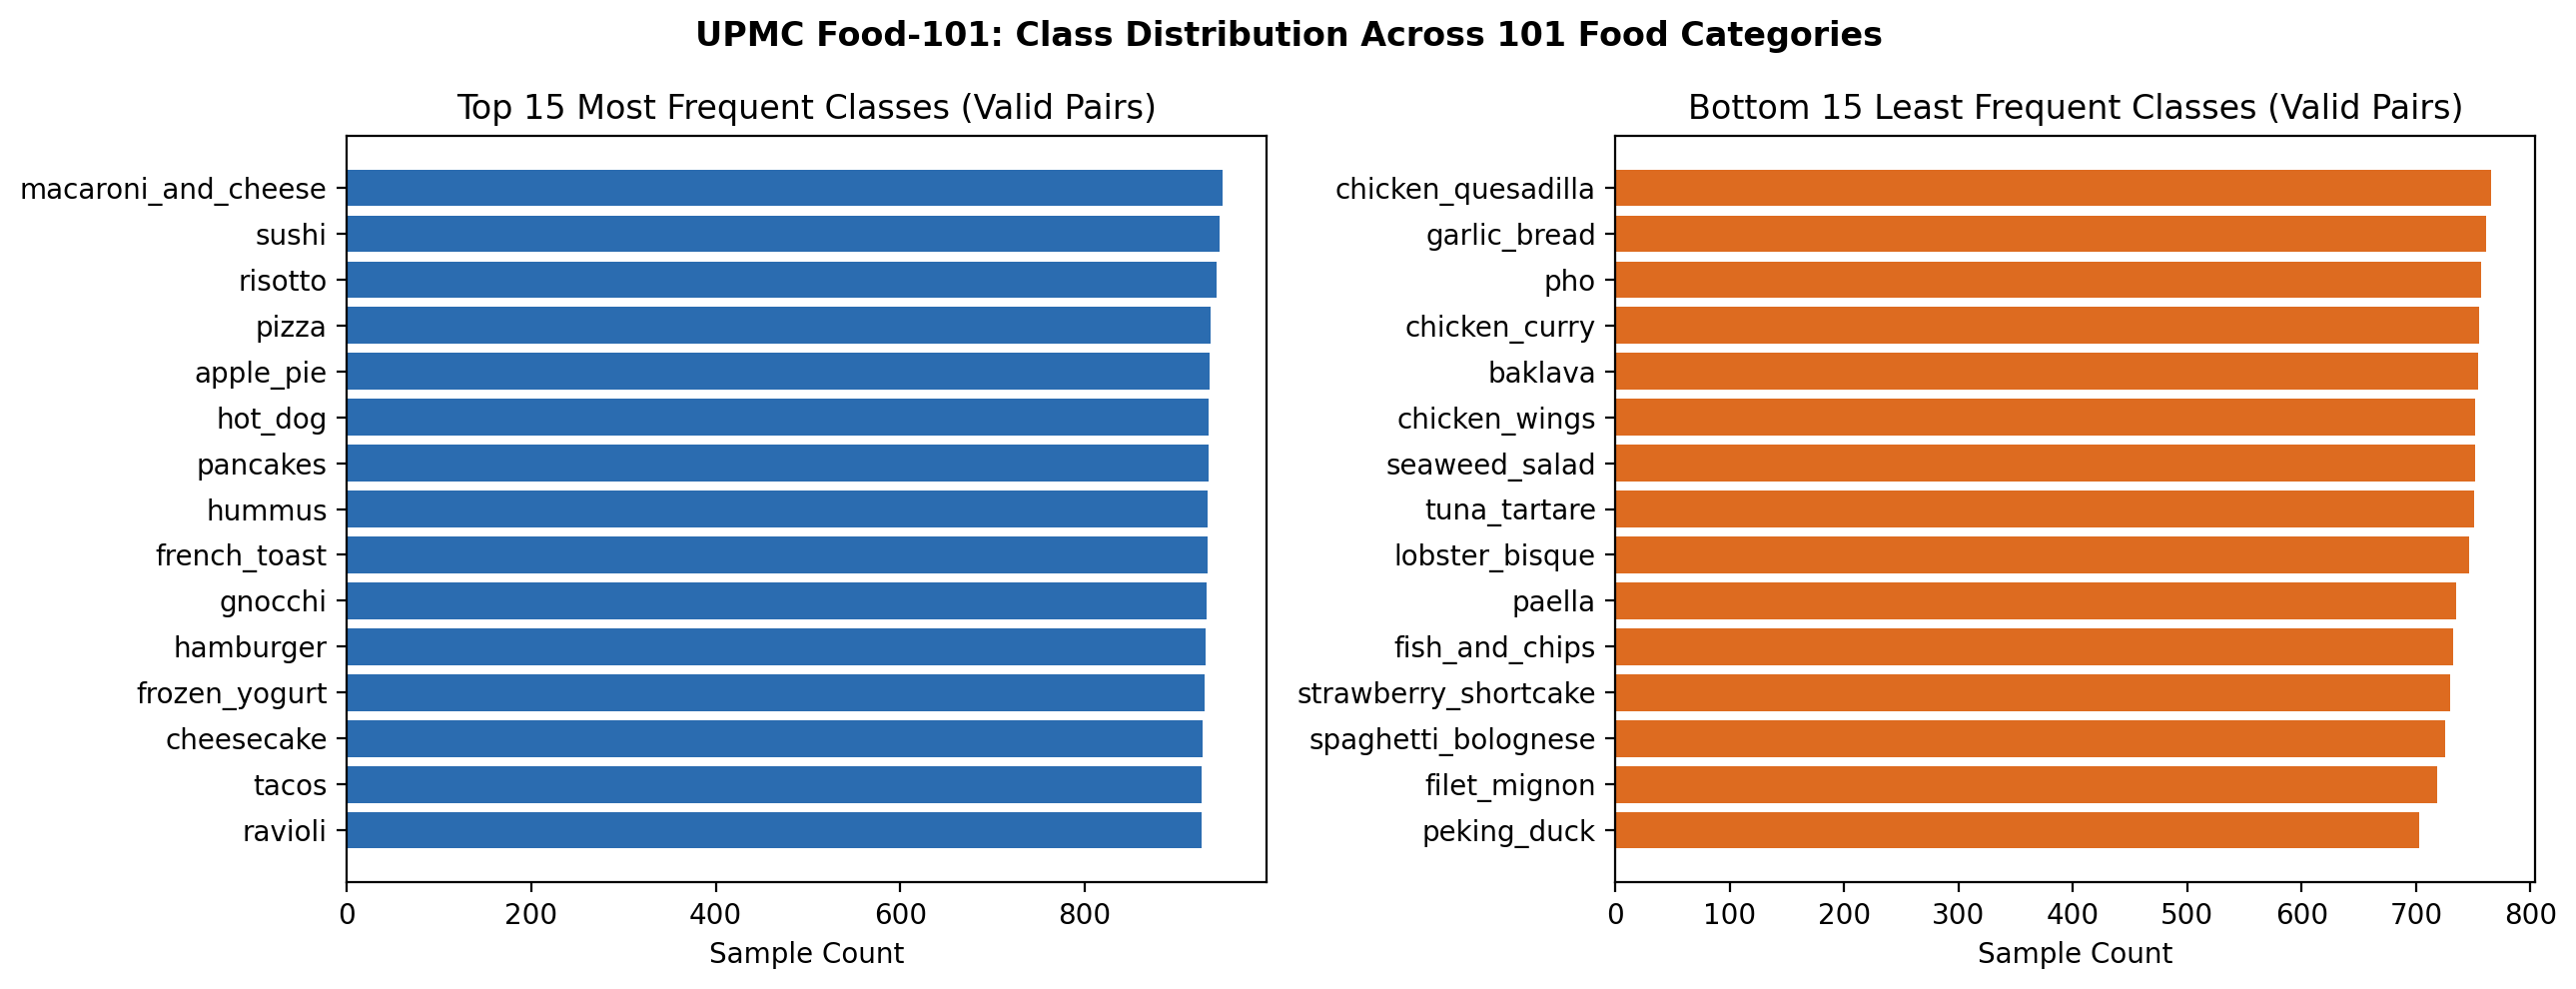
\includegraphics[width=0.92\linewidth]{../outputs/a3_eda/figures/class_distribution.png}
    \caption{Top-15 and Bottom-15 class counts (703 for \texttt{peking\_duck} to 950 for \texttt{macaroni\_and\_cheese}; $1.35\times$ ratio).}
\end{figure}

\begin{figure}[H]
    \centering
    \begin{minipage}{0.49\linewidth}
        \centering
        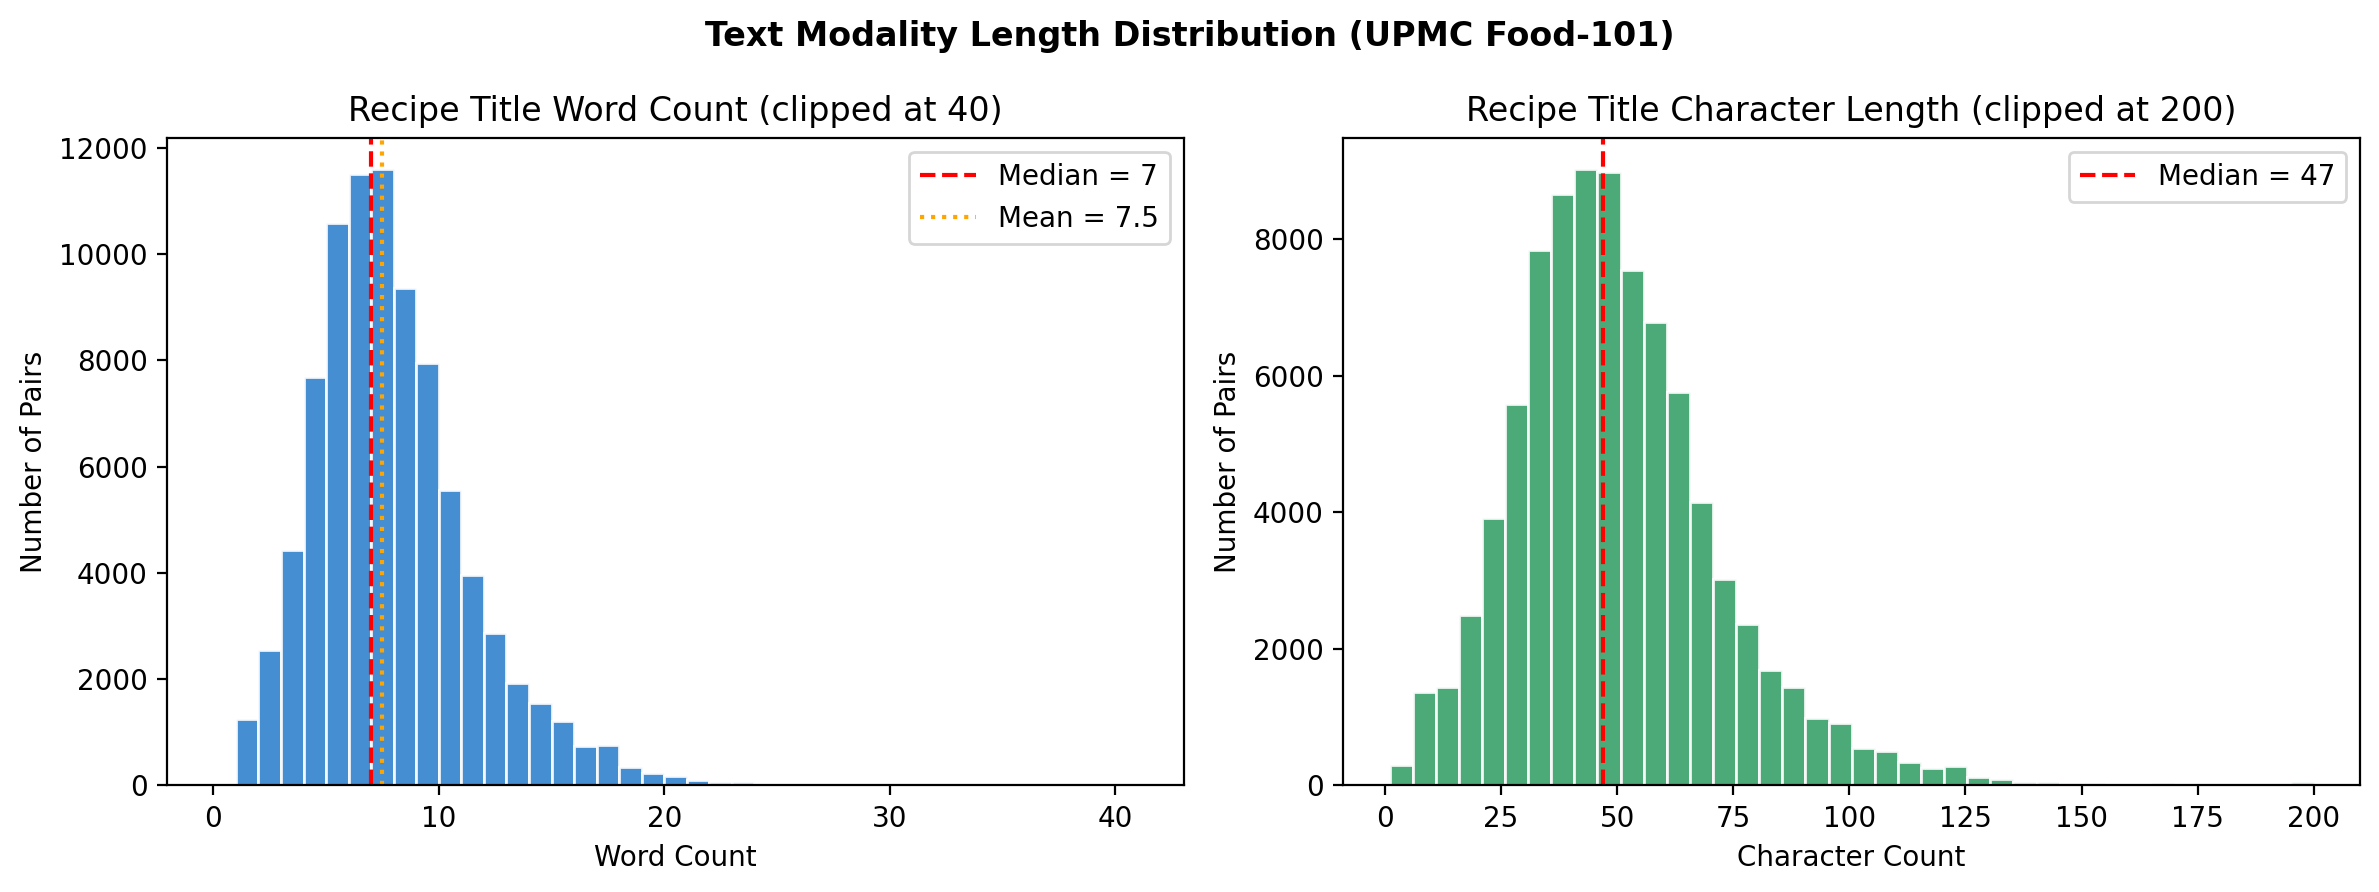
\includegraphics[width=\linewidth]{../outputs/a3_eda/figures/text_length_distribution.png}
        \caption{Recipe title word and character length distributions.}
    \end{minipage}\hfill
    \begin{minipage}{0.49\linewidth}
        \centering
        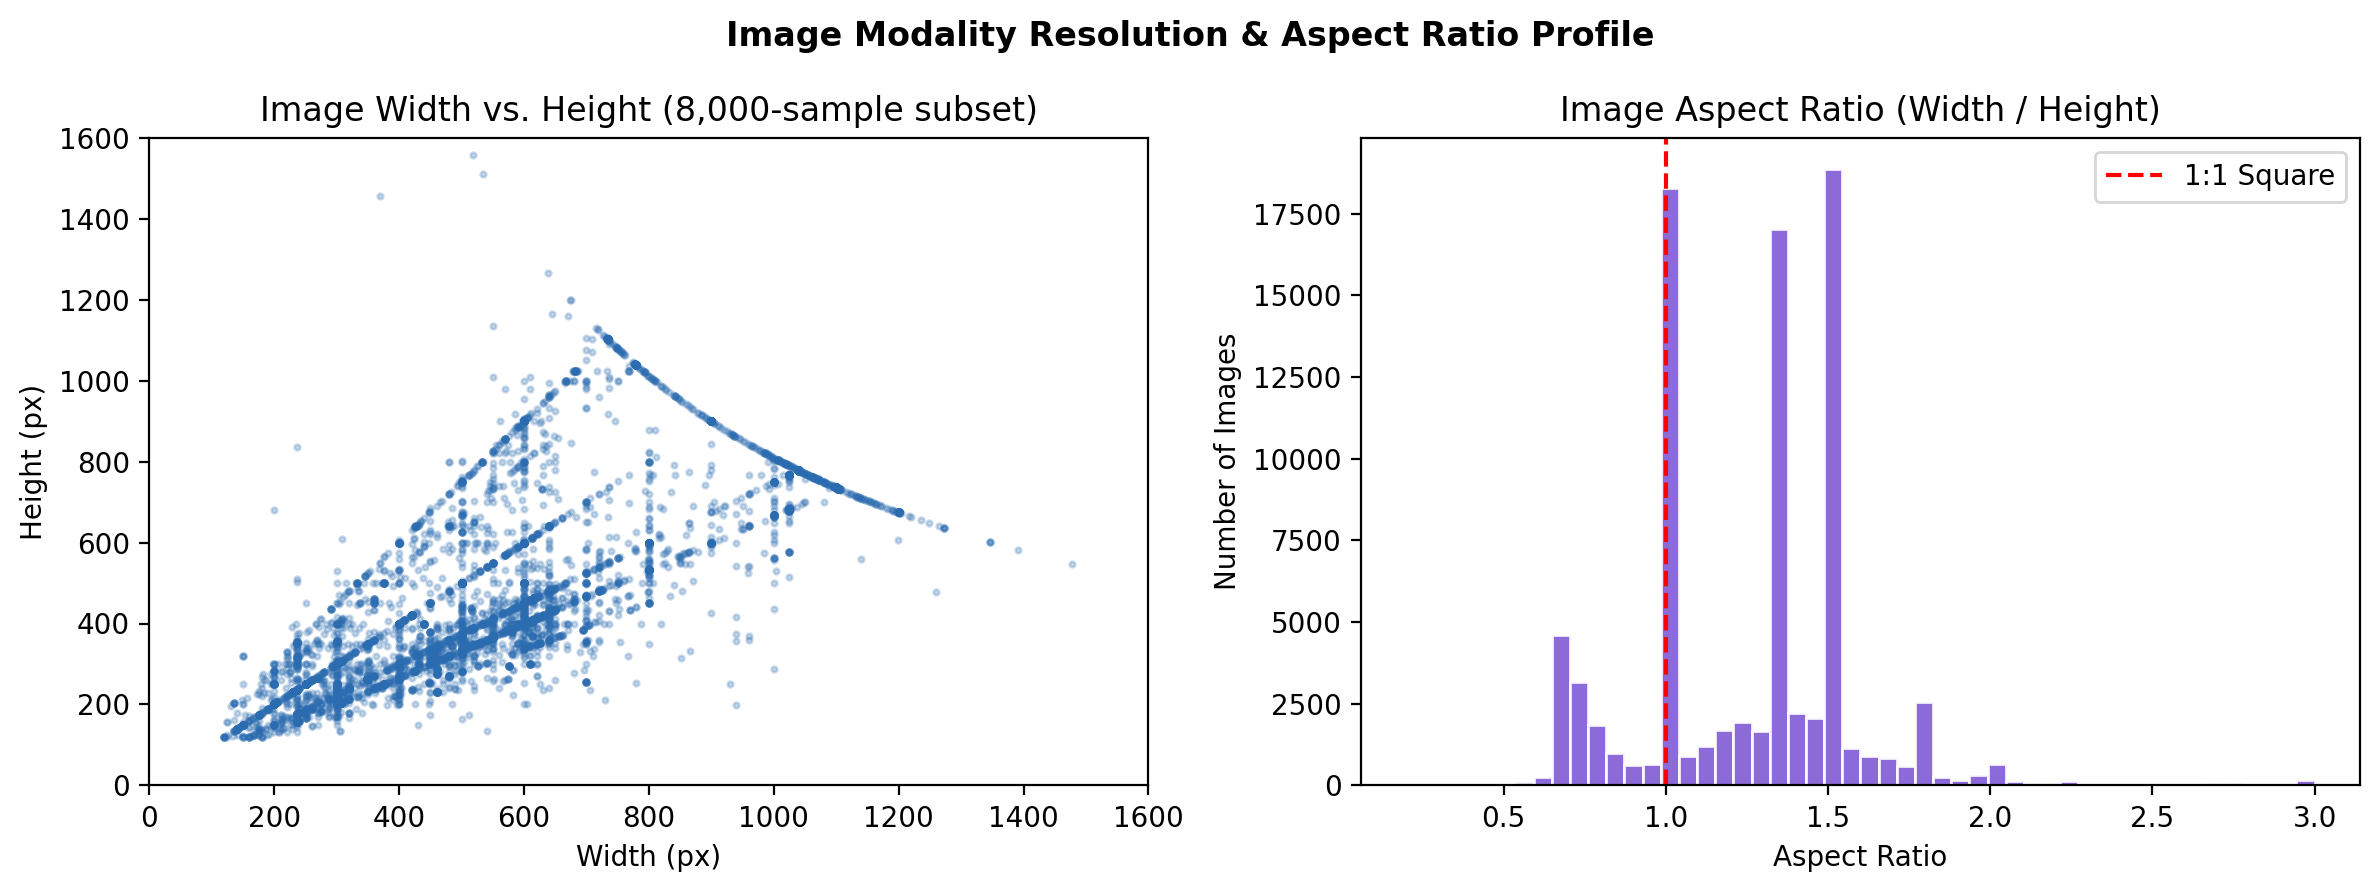
\includegraphics[width=\linewidth]{../outputs/a3_eda/figures/image_dimensions.png}
        \caption{Image resolution scatter and aspect-ratio profile.}
    \end{minipage}
\end{figure}

\begin{figure}[H]
    \centering
    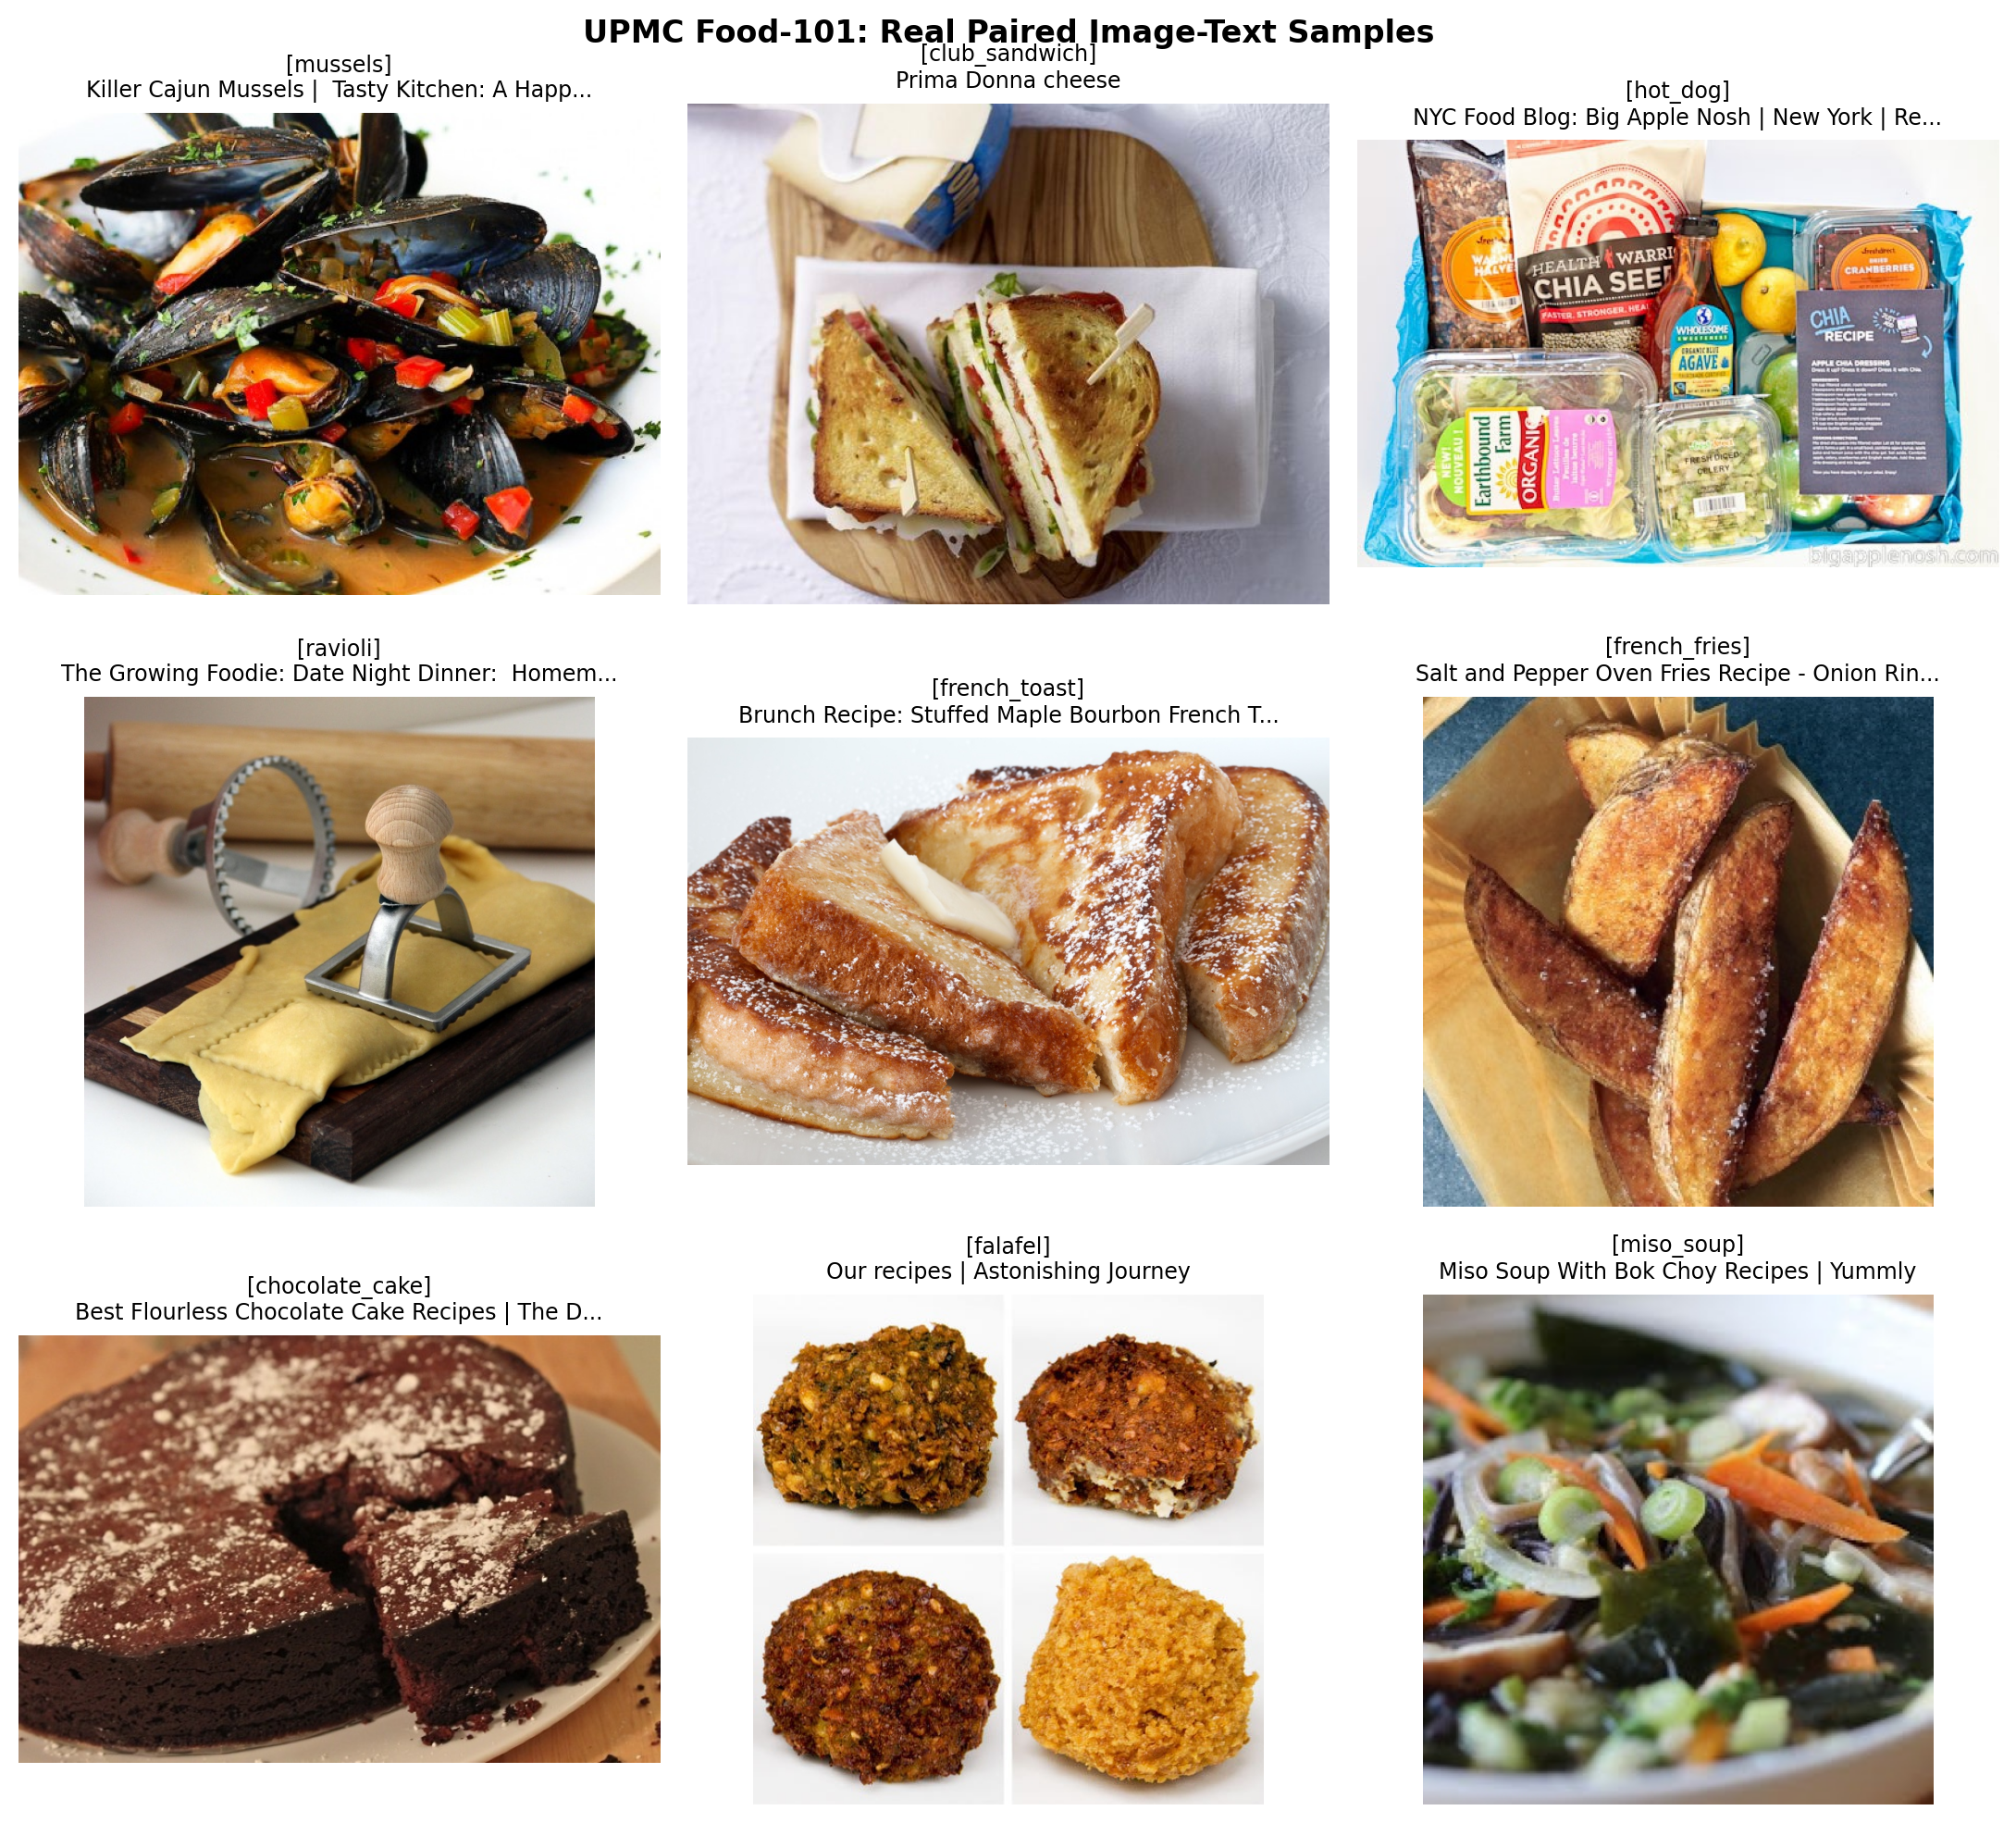
\includegraphics[width=0.82\linewidth]{../outputs/a3_eda/figures/sample_pairs_preview.png}
    \caption{Representative paired $(\text{Image}, \text{Recipe Title}, \text{Class})$ examples from UPMC Food-101.}
\end{figure}

\section{Split Plan \& Leakage-Prevention Unit}

\begin{itemize}
    \item \textbf{Leakage-Prevention Unit:} \texttt{recipe\_id} (pairing image and title from a single recipe webpage), further clustered into equivalence groups by \textbf{exact SHA-256 hash} and \textbf{perceptual dHash (Hamming distance $\le 3$)} via Union-Find so duplicate or near-duplicate images never straddle \texttt{train} and \texttt{val}.
    \item \textbf{Split Method:} \texttt{StratifiedGroupKFold(n\_splits=5, shuffle=True, random\_state=42)} on the 65,085 official training pairs, keeping the 21,683 official test pairs untouched for final evaluation.
\end{itemize}

\begin{table}[H]
\centering
\caption{Leakage-Controlled Dataset Partitions (\texttt{outputs/a3\_eda/splits/})}
\begin{tabularx}{\linewidth}{l r r c c X}
\toprule
\textbf{Split} & \textbf{Samples} & \textbf{Classes} & \textbf{Word Mean / Med} & \textbf{Class-in-Text} & \textbf{Split File} \\
\midrule
Train (80\%) & 52,068 & 101 & 7.54 / 7.0 & 72.11\% & \texttt{splits/train.csv} \\
Validation (20\%) & 13,017 & 101 & 7.55 / 7.0 & 71.93\% & \texttt{splits/val.csv} \\
Test (Official) & 21,683 & 101 & 7.36 / 7.0 & 72.08\% & \texttt{splits/test.csv} \\
\bottomrule
\end{tabularx}
\end{table}

\textbf{Leakage Audit:} Zero exact SHA-256 and zero near-duplicate dHash overlaps exist between \texttt{train} and \texttt{val}, with validation shares per class tightly bounded between \textbf{19.85\% and 20.12\%}. Auditing official \texttt{test} against \texttt{train+val} revealed \textbf{1,018} exact SHA-256 overlaps (825 train--test, 193 val--test) and \textbf{4,395} near-duplicate pairs. In M2/M3, we will report metrics on both the full official test set (21,683) and a \textbf{de-duplicated clean test subset} excluding overlapping hashes.

\begin{figure}[H]
    \centering
    \begin{minipage}{0.49\linewidth}
        \centering
        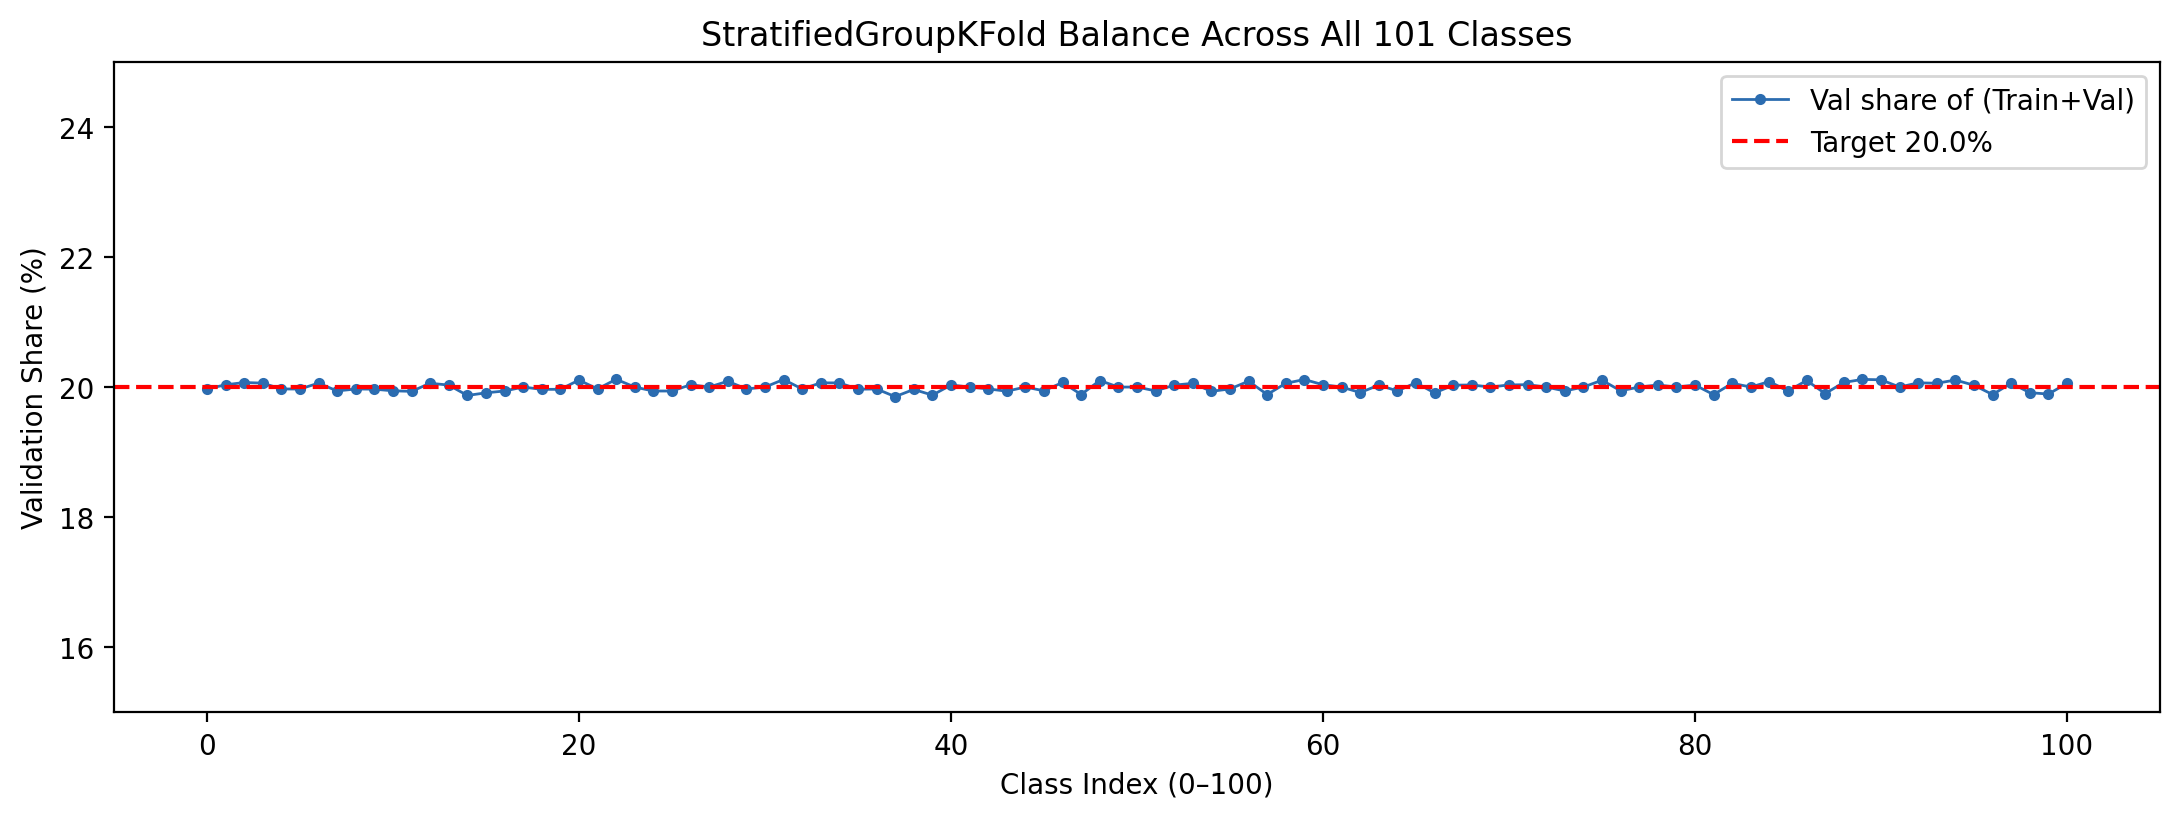
\includegraphics[width=\linewidth]{../outputs/a3_eda/figures/split_class_prevalence.png}
        \caption{Validation share across all 101 classes (19.85\%--20.12\%).}
    \end{minipage}\hfill
    \begin{minipage}{0.49\linewidth}
        \centering
        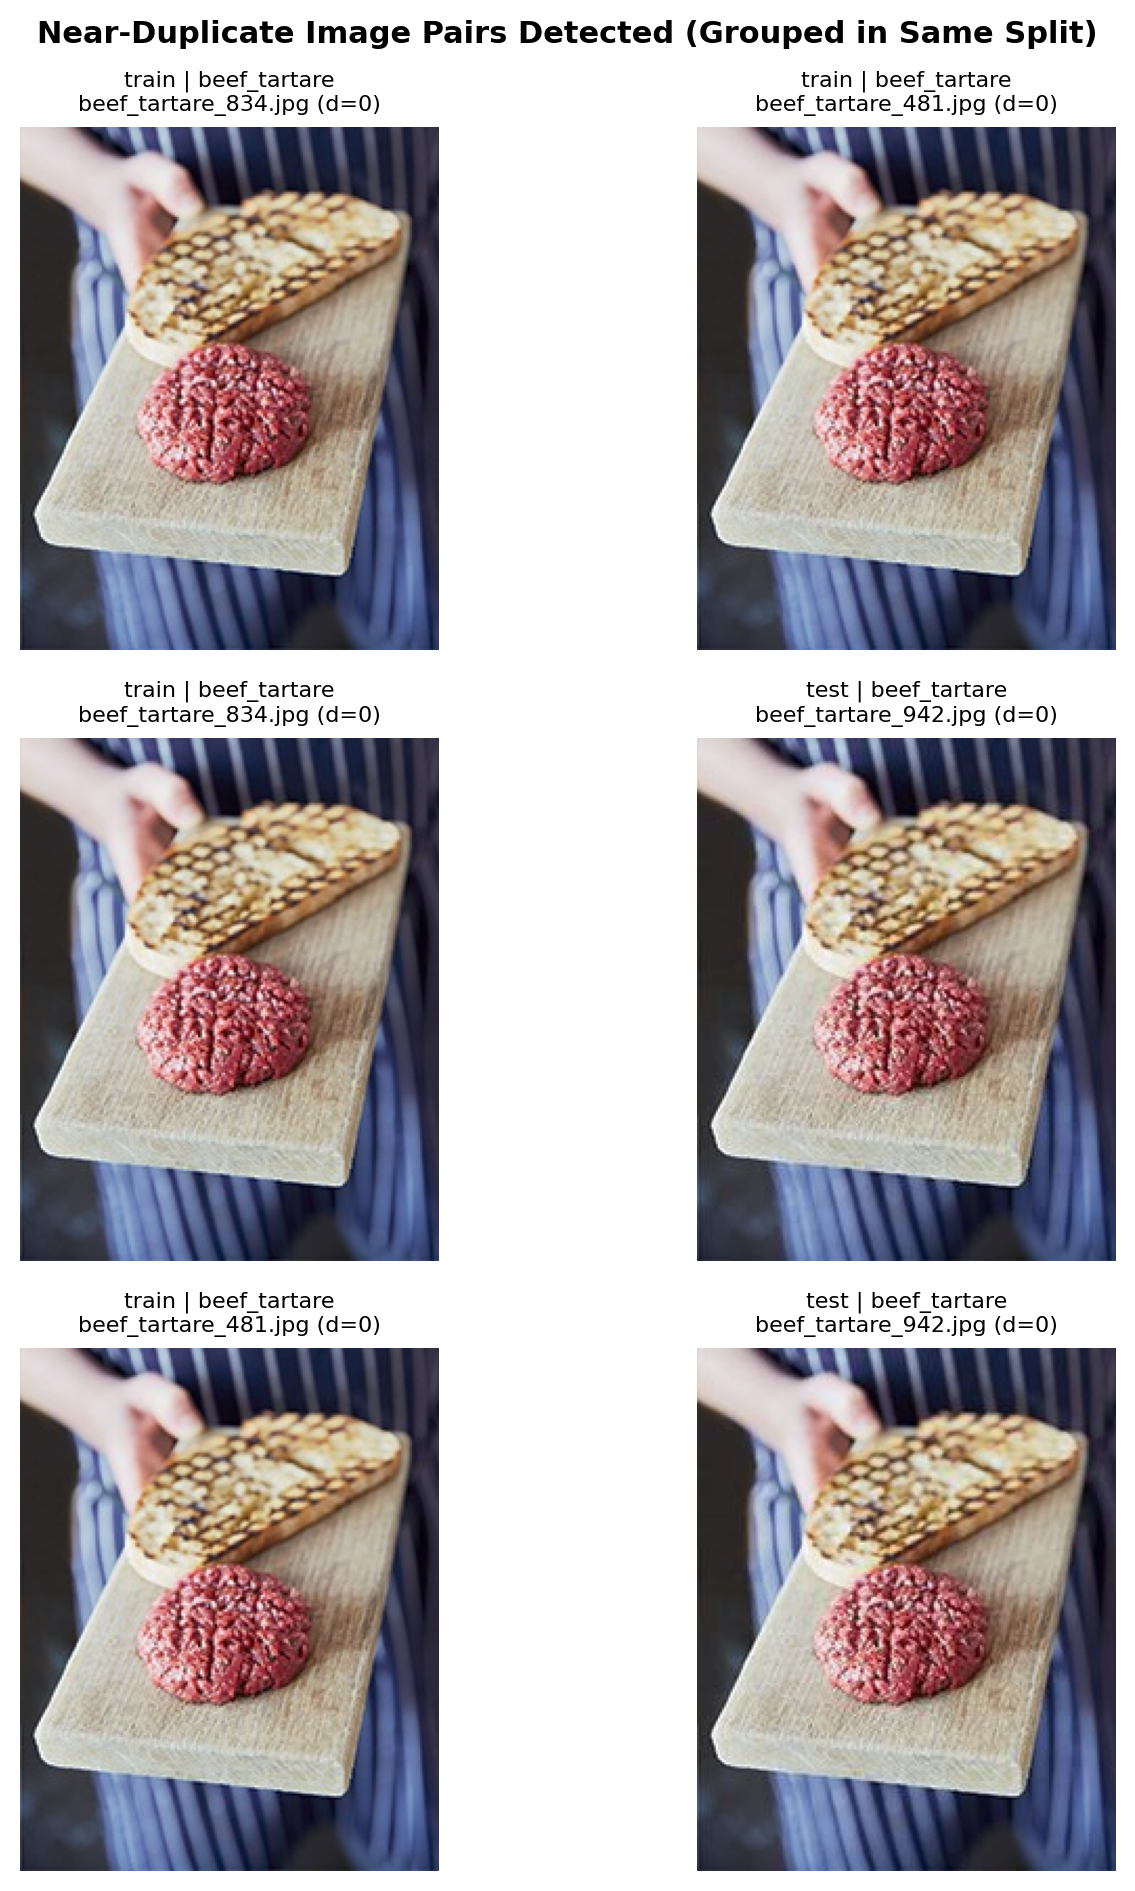
\includegraphics[width=\linewidth]{../outputs/a3_eda/figures/near_duplicate_preview.png}
        \caption{Near-duplicate image pairs grouped in the same split.}
    \end{minipage}
\end{figure}

\section{Planned Models, Metrics \& Ablation Study}

\subsection{\textbf{Evaluation Metrics (Handbook Section 29.3)}}
Primary evaluation metrics are \textbf{Top-1 Accuracy} and \textbf{Macro-F1} across all 101 classes, with \textbf{Top-5 Accuracy} reported as a secondary metric to diagnose fine-grained dish confusion.

\subsection{\textbf{Four Mandatory Models (Handbook Sections 29.1 \& 29.2)}}
All four configurations share identical splits, preprocessing (\texttt{html.unescape()}, RGB $224\times 224$), random seed (42), AdamW optimizer, and cosine learning-rate schedule:

\begin{table}[H]
\centering
\caption{Planned Unimodal Baselines, Simple Fusion, and Improved Multimodal Model}
\begin{tabularx}{\linewidth}{c l X X}
\toprule
\textbf{\#} & \textbf{Model Role} & \textbf{Architecture \& Fusion Design} & \textbf{Loss \& Training Protocol} \\
\midrule
1 & Unimodal A (Image) & \texttt{ConvNeXt-Tiny} (ImageNet-1K) + linear head & Cross-Entropy, 10 epochs, FP16 \\
2 & Unimodal B (Text) & \texttt{DistilBERT-base-uncased} (\texttt{max\_len=64}) + \texttt{[CLS]} head & Cross-Entropy, 6 epochs, FP16 \\
3 & Simple Fusion & Late concatenation $[h_{\text{img}}; h_{\text{txt}}] \in \mathbb{R}^{1536} \to$ LayerNorm + Dropout + MLP & Joint Cross-Entropy, end-to-end \\
4 & Improved Multimodal & \textbf{Gated Cross-Modal Attention} (512-d shared space, gate $g = \sigma(W[h_v; h_t])$) + \textbf{Modality Dropout ($p=0.15$)} & $\mathcal{L} = \mathcal{L}_{\text{mm}} + 0.2\,\mathcal{L}_{\text{img}} + 0.2\,\mathcal{L}_{\text{txt}}$; differential LR \\
\bottomrule
\end{tabularx}
\end{table}

\subsection{\textbf{Ablation \& Modality Interaction Plan (Handbook Section 30)}}
\begin{itemize}
    \item \textbf{Ablation 1 (Modality Removal):} Compare Image-only vs.\ Text-only vs.\ Simple Concatenation vs.\ Gated Cross-Attention.
    \item \textbf{Ablation 2 (Fusion Regularization):} Quantify the effect of Modality Dropout ($p=0.15$) and auxiliary unimodal losses on noisy-title samples (e.g., \texttt{\#NAME?} or titles omitting the dish name).
    \item \textbf{Support vs.\ Conflict Analysis:} Categorize test predictions into modality-support cases (both modalities reinforce or disambiguate) and modality-conflict cases (misleading web title vs.\ clear dish photograph).
\end{itemize}

\section{Compute Estimate \& Subset Rules}

\begin{table}[H]
\centering
\caption{Google Colab T4 (16 GB VRAM, FP16 AMP) Compute Estimate}
\begin{tabularx}{\linewidth}{X l c r}
\toprule
\textbf{Configuration} & \textbf{Hardware} & \textbf{Batch / Precision} & \textbf{Est. GPU-Hours} \\
\midrule
Unimodal Image (\texttt{ConvNeXt-Tiny}, 10 ep) & Colab T4 (16 GB) & 64 / FP16 AMP & $\sim 2.5$ h \\
Unimodal Text (\texttt{DistilBERT}, 6 ep) & Colab T4 (16 GB) & 128 / FP16 AMP & $\sim 0.5$ h \\
Simple Fusion (10 ep) & Colab T4 (16 GB) & 64 / FP16 AMP & $\sim 3.0$ h \\
Improved Multimodal + Ablations (2--3 runs) & Colab T4 (16 GB) & 64 / FP16 AMP & $\sim 6.0$ h \\
\midrule
\textbf{Total M2 + M3 Budget} & \multicolumn{2}{l}{Full dataset (52,068 train / 13,017 val / 21,683 test)} & \textbf{$\sim 12.0$ h} \\
\bottomrule
\end{tabularx}
\end{table}

\noindent\textbf{Subset Rules:} All 4 main models will be trained and evaluated on the full leakage-controlled dataset. Rapid debugging or sanity checks may use a deterministic 20\% stratified subset (\texttt{seed=42}).

\section{AI Usage Disclosure \& References}

\begin{itemize}
    \item \textbf{AI Usage Disclosure (Handbook Section 5.2):} AI coding assistant (Antigravity / Gemini) was used to draft the EDA notebook (\texttt{notebooks/A3\_EDA\_Proposal.ipynb}), structure \texttt{assignment3.md}, and format this LaTeX report. All 86,768 image/text integrity checks, SHA-256/dHash duplicate audits, \texttt{StratifiedGroupKFold} splits, and figures were executed locally on the real \texttt{UPMC-Food-101.zip} archive and verified against \texttt{outputs/a3\_eda/summary.json} and \texttt{quality\_checks.json}.
\end{itemize}

\begin{thebibliography}{9}
\bibitem{wang2015} Wang, X., Kumar, D., Thome, N., Cord, M., \& Precioso, F. (2015). \emph{Recipe Recognition with Large Multimodal Food Dataset}. IEEE ICMEW.
\bibitem{liu2022} Liu, Z., Mao, H., Wu, C.-Y., Feichtenhofer, C., Darrell, T., \& Xie, S. (2022). \emph{A ConvNet for the 2020s}. CVPR.
\bibitem{sanh2019} Sanh, V., Debut, L., Chaumond, J., \& Wolf, T. (2019). \emph{DistilBERT, a distilled version of BERT: smaller, faster, cheaper and lighter}. NeurIPS EMC2 Workshop.
\end{thebibliography}

\end{document}
